\documentclass[12pt]{beamer}
\usepackage{../Estilos/BeamerMAF}
\usetheme{Warsaw}
\usecolortheme{seahorse}
%\useoutertheme{default}
\setbeamercovered{invisible}
% or whatever (possibly just delete it)
\setbeamertemplate{section in toc}[sections numbered]
\setbeamertemplate{subsection in toc}[subsections numbered]
\setbeamertemplate{subsection in toc}{\leavevmode\leftskip=3.2em\rlap{\hskip-2em\inserttocsectionnumber.\inserttocsubsectionnumber}\inserttocsubsection\par}
\setbeamercolor{section in toc}{fg=blue}
\setbeamercolor{subsection in toc}{fg=blue}
\setbeamercolor{frametitle}{fg=blue}
\setbeamertemplate{caption}[numbered]

\setbeamertemplate{footline}
\beamertemplatenavigationsymbolsempty
\setbeamertemplate{headline}{}


\makeatletter
\setbeamercolor{section in foot}{bg=gray!30, fg=black!90!orange}
\setbeamercolor{subsection in foot}{bg=blue!30}
\setbeamercolor{date in foot}{bg=black}
\setbeamertemplate{footline}
{
  \leavevmode%
  \hbox{%
  \begin{beamercolorbox}[wd=.333333\paperwidth,ht=2.25ex,dp=1ex,center]{section in foot}%
    \usebeamerfont{section in foot} \insertsection
  \end{beamercolorbox}%
  \begin{beamercolorbox}[wd=.333333\paperwidth,ht=2.25ex,dp=1ex,center]{subsection in foot}%
    \usebeamerfont{subsection in foot}  \insertsubsection
  \end{beamercolorbox}%
  \begin{beamercolorbox}[wd=.333333\paperwidth,ht=2.25ex,dp=1ex,right]{date in head/foot}%
    \usebeamerfont{date in head/foot} \insertshortdate{} \hspace*{2em}
    \insertframenumber{} / \inserttotalframenumber \hspace*{2ex} 
  \end{beamercolorbox}}%
  \vskip0pt%
}
\makeatother

\makeatletter
\patchcmd{\beamer@sectionintoc}{\vskip1.5em}{\vskip0.8em}{}{}
\makeatother

\newlength{\depthofsumsign}
\setlength{\depthofsumsign}{\depthof{$\sum$}}
\newcommand{\nsum}[1][1.4]{% only for \displaystyle
    \mathop{%
        \raisebox
            {-#1\depthofsumsign+1\depthofsumsign}
            {\scalebox
                {#1}
                {$\displaystyle\sum$}%
            }
    }
}
\def\scaleint#1{\vcenter{\hbox{\scaleto[3ex]{\displaystyle\int}{#1}}}}
\def\scaleoint#1{\vcenter{\hbox{\scaleto[3ex]{\displaystyle\oint}{#1}}}}
\def\bs{\mkern-12mu}

\makeatletter
\setbeamertemplate{footline}
{
  \leavevmode%
  \hbox{%
  \begin{beamercolorbox}[wd=.333333\paperwidth,ht=2.25ex,dp=1ex,center]{section in foot}%
    \usebeamerfont{section in foot} \insertsection
  \end{beamercolorbox}%
  \begin{beamercolorbox}[wd=.333333\paperwidth,ht=2.25ex,dp=1ex,center]{subsection in foot}%
    \usebeamerfont{subsection in foot}  \insertsubsection
  \end{beamercolorbox}%
  \begin{beamercolorbox}[wd=.333333\paperwidth,ht=2.25ex,dp=1ex,right]{date in head/foot}%
    \usebeamerfont{date in head/foot} {Material adicional} \hspace*{2em}
    \insertframenumber{} / \inserttotalframenumber \hspace*{2ex} 
  \end{beamercolorbox}}%
  \vskip0pt%
}
\makeatother
\makeatletter
\patchcmd{\beamer@sectionintoc}{\vskip1.5em}{\vskip0.8em}{}{}
\makeatother

\title{\large{Ejercicios}}
\subtitle{Funciones Gamma y Beta}
\author{M. en C. Gustavo Contreras Mayén}
\date{}
\institute{Facultad de Ciencias - UNAM}
\titlegraphic{
\includegraphics[width=1.75cm]{../Imagenes/escudo-facultad-ciencias}\hspace*{4.75cm}~%
   
\includegraphics[width=1.75cm]{../Imagenes/escudo-unam}
}
\setbeamertemplate{navigation symbols}{}
\begin{document}
\maketitle
\fontsize{14}{14}\selectfont
\spanishdecimal{.}
\section*{Contenido}
\frame[allowframebreaks]{\tableofcontents[currentsection, hideallsubsections]}

\section{Función Gamma}
\frame{\tableofcontents[currentsection, hideothersubsections]}

\subsection{Ejemplo de la mecánica}

\begin{frame}
\frametitle{Ejercicio}
Una partícula de masa $m$ en el eje $x$ positivo es atraída hacia el origen por una fuerza variable tal que el producto de la magnitud de la fuerza por la distancia desde el origen es una constante $k$. La partícula parte del reposo en $x = L$.
\\
\bigskip
\pause
\textbf{Determina el tiempo necesario para que la partícula llegue el origen}.
\end{frame}
\begin{frame}
\frametitle{Representando el problema}
Con un esquema tenemos que nuestro problema es:
\begin{figure}
    \centering
    \includestandalone{Figuras/Ejercicio_Gamma_Particula}
    \caption{La partícula desplazándose hacia el origen.}
\end{figure}
\end{frame}
\begin{frame}
\frametitle{Solución}
Partimos de la segunda ley de Newton $F = m \, a$, donde tenemos que la única componente que permanece está en la dirección del eje $x$.
\\
\bigskip
\pause
Entonces tenemos que
\begin{align*}
- \dfrac{k}{x} = m \, \dv[2]{x}{t}
\end{align*}
\end{frame}
\begin{frame}
\frametitle{Manejo algebraico}
Acomodemos los términos y multipliquemos ambos lados por $\dv*{x}{t}$:
\begin{align*}
m \left( \dv[2]{x}{t} \right) \left( \dv{x}{t} \right) = - \dfrac{k}{x} \,  \left( \dv{x}{t} \right)
\end{align*}
\pause
Antes de integrar ambos lados de la igualdad, expresemos una derivada de manera conveniente:
\end{frame}
\begin{frame}
\frametitle{Representación de una derivada}
Tomemos en cuenta que la derivada:
\begin{align*}
\left[ \left( \dv{x}{t} \right)^{2} \right]^{\prime} = 2 \, \left( \dv{x}{t} \right) \left( \dv[2]{x}{t} \right)
\end{align*}
\pause
Al integrar ambos lados de la igualdad, nos queda por resolver:
\begin{align*}
\dfrac{1}{2} \, m \, \left( \dv{x}{t} \right)^{2} = - k \int_{L}^{x} \dfrac{\left( \dv{x}{t} \right)}{x} \dd{t}
\end{align*}
\end{frame}
\begin{frame}
\frametitle{Resolviendo la integral}
Se tiene entonces que:
\begin{eqnarray*}
\dfrac{1}{2} \, m \, \left( \dv{x}{t} \right)^{2} &=& - k \int_{L}^{x} \dfrac{\left( \dv{x}{t} \right)}{x} \dd{t} \\[0.5cm] \pause
&=& - k \, \ln(x) + k \, \ln(L)
\end{eqnarray*}
\pause
Vemos que esta ecuación hace que:
\begin{align*}
\dv{x}{t} = 0 \hspace{1cm} \mbox{cuando } x = L
\end{align*}
en concordancia con la condición de frontera.
\end{frame}
\begin{frame}
\frametitle{Resolviendo la ecuación}
Resolvemos la ecuación para la velocidad $\dv*{x}{t}$:
\begin{eqnarray*}
\dfrac{1}{2} \, m \, \left( \dv{x}{t} \right)^{2} &=& - k \, \ln(x) + k \, \ln(L) \\[0.5em] \pause
\left( \dv{x}{t} \right)^{2} &=& \dfrac{2 \, k}{m} \ln(\dfrac{L}{x}) \\[0.em] \pause
\dv{x}{t} &=& - \sqrt{\dfrac{2 \, k}{m} \ln(\dfrac{L}{x})} \\[0.em] \pause
\dd{t} &=& - \sqrt{\dfrac{m}{2 \, k}} \left[ \ln(\dfrac{L}{x}) \right]^{-\frac{1}{2}}
\end{eqnarray*}
\end{frame}
\begin{frame}
\frametitle{Resolviendo la ecuación}
Tomamos el valor negativo de la raíz cuadrada ya que el movimiento se presenta en la dirección negativa del eje $x$.
\\
\bigskip
\pause
Al haber separado las variables, ya podemos integrar:
\begin{align*}
t = - \sqrt{\dfrac{m}{2 \, k}} \int_{L}^{0} \left[ \ln(\dfrac{L}{x}) \right]^{-\frac{1}{2}} \dd{x}
\end{align*}
\pause
Al parecer se complica con respecto a la integración!
\end{frame}
\begin{frame}
\frametitle{Uso de una identidad}
Vamos a ocupar la siguiente identidad:
\begin{align}
\int_{0}^{\infty} t^{a} \, \exp(-b \, t^{c}) \dd{t} = \dfrac{\Gamma \left( \dfrac{a + 1}{c} \right)}{c \, b^{(a+1)/c}}
\label{eq:identidad_Gamma}
\end{align}
donde $b$ y $c$ son constantes positivas, mientras que $a$ es una constante tal que $a > - 1$.
\end{frame}
\begin{frame}
\frametitle{Otro resultado}
Consideremos la siguiente integral:
\begin{align*}
\int_{0}^{1} x^{m} \, \left( \ln \dfrac{1}{x} \right)^{n} \dd{x} \hspace{1cm} m > -1, n > -1
\end{align*}
\pause
Hacemos el siguiente cambio de variable:
\begin{align*}
\ln \left(\dfrac{1}{x} \right) = t
\end{align*}
\end{frame}
\begin{frame}
\frametitle{Otro resultado}
Con el cambio de variable tenemos que:
\begin{align*}
\dfrac{1}{x} &= e^{t} \\[0.5em]
x &= e^{-t} \\[0.5em]
x^{m} &= e^{-m t} \\[0.5em]
\dd{x} &= - e^{-t} \dd{t}
\end{align*}
\end{frame}
\begin{frame}
\frametitle{Otro resultado}
Entonces al reexpresar la integral con el cambio de variable y considerando que al invertir los límites de integración, se cancela el signo negativo, tendremos que:
\begin{align*}
\int_{0}^{1} x^{m} \, \left( \ln \dfrac{1}{x} \right)^{n} \dd{x} = \int_{0}^{\infty} t^{n} \, \exp \big[-(m + 1) \, t \big] \dd{t}
\end{align*}
\end{frame}
\begin{frame}
\frametitle{Usando el resultado}
Utilizando la propiedad (\ref{eq:identidad_Gamma}), con $a = n$, $b = m + 1$ y $c = 1$, el valor de la integral es:
\begin{align}
\int_{0}^{1} x^{m} \, \left( \ln \dfrac{1}{x} \right)^{n} \dd{x} = \dfrac{\Gamma (n + 1)}{(m + 1)^{n+1}}
\label{eq:ecuacion_propiedad_Gamma}
\end{align}
\end{frame}
\begin{frame}
\frametitle{Regresando al problema}
Una vez revisados los dos resultados anteriores, para el problema de la partícula moviéndose al origen, entonces hacemos el cambio de variable $x = L \, u$ para obtener:
\begin{align*}
t &= - \sqrt{\dfrac{m}{2 \, k}} \int_{L}^{0} \left[ \ln(\dfrac{L}{x}) \right]^{-\frac{1}{2}} \dd{x} \\[0.5em]
t &= L \, \sqrt{\dfrac{m}{2 \, k}} \, \int_{0}^{1} u^{0} \, \left( \ln \dfrac{1}{u} \right)^{-1/2} \dd{u}
\end{align*}
\end{frame}
\begin{frame}
\frametitle{Solución}
Del resultado obtenido en la ec. (\ref{eq:ecuacion_propiedad_Gamma})
\begin{align*}
\int_{0}^{1} x^{m} \, \left( \ln \dfrac{1}{x} \right)^{n} \dd{x} = \dfrac{\Gamma (n + 1)}{(m + 1)^{n+1}}
\end{align*}    
\pause
\begin{align*}
t &= L \, \sqrt{\dfrac{m}{2 \, k}} \, \int_{0}^{1} u^{0} \, \left( \ln \dfrac{1}{u} \right)^{-1/2} \dd{u}
\end{align*}
Entonces tenemos que: $m = 0$ y $n = -1/2$.
\end{frame}
\begin{frame}
\frametitle{Solución}
Por lo que:
\begin{eqnarray*}
t &=& L \, \sqrt{\dfrac{m}{2 \, k}} \, \Gamma(-1/2 + 1) = \\[0.5em] \pause
&=& L \, \sqrt{\dfrac{m}{2 \, k}} \, \Gamma(1/2) = \\[0.5em] \pause
&=& L \, \sqrt{\dfrac{m}{2 \, k}} \, \sqrt{\pi} = \\[0.5em] \pause
t &=& L \, \sqrt{\dfrac{m \, \pi}{2 \, k}} \qed
\end{eqnarray*}
\end{frame}

\section{Función Beta}
\frame{\tableofcontents[currentsection, hideothersubsections]}
\subsection{Ejercicio de la geometría}


\begin{frame}
\frametitle{Enunciado del problema}
En la siguiente figura (\ref{fig:figura_curva_estrella}) se aprecia la curva determinada por la expresión
\begin{align}
x^{b/c} + y^{b/c} = a^{b/c}
\label{eq:ecuacion_curva_estrella}
\end{align}
donde: $a$ es una constante positiva, $b$ es un entero par positivo y $c$ es un entero impar positivo.
\end{frame}
\begin{frame}
\frametitle{Enunciado del problema}
\begin{figure}[H]
    \centering
    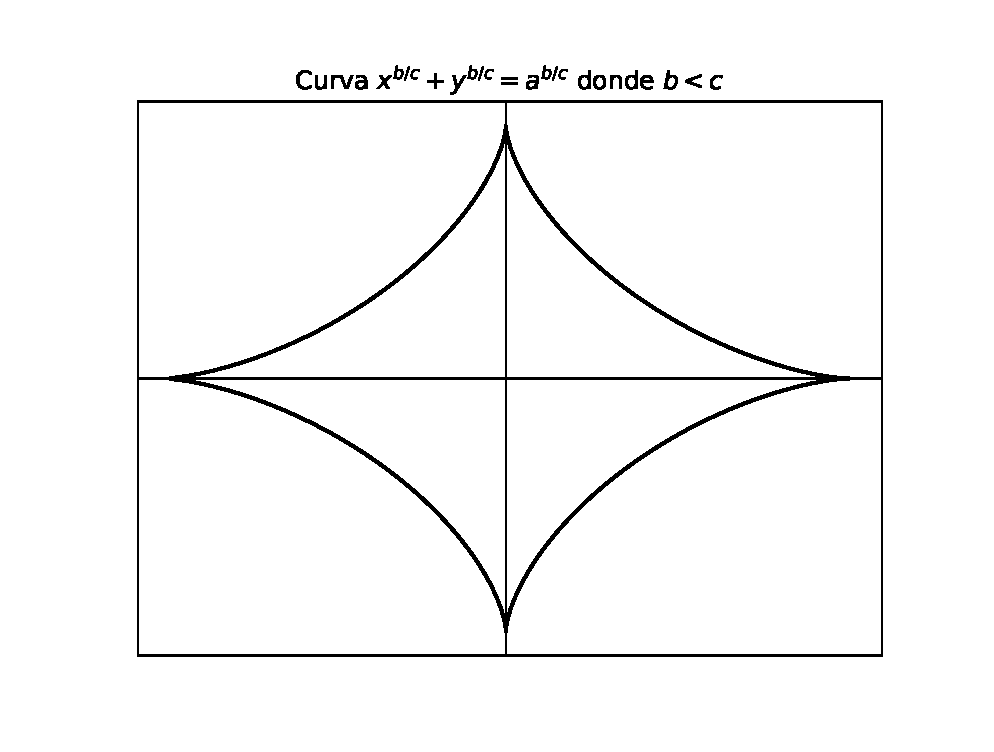
\includegraphics[scale=0.5]{Imagenes/plot_curva_estrella_01.eps}
    \caption{Estrella con cuatro picos cóncavos.}
    \label{fig:figura_curva_estrella}
\end{figure}
\end{frame}
\begin{frame}
\frametitle{Enunciado del problema}
Calcula el área dentro de la curva (ec. \ref{eq:ecuacion_curva_estrella}) en términos de la función Gamma cuando el exponente $b/c$ es $2/3$.
\\
\bigskip
\pause
El enunciado nos pide el resultado en términos de la función Gamma, cuando en esta sección veremos la función Beta\pause, entonces habrá que ocupar la relación que vincula la función Gamma con la Beta.
\end{frame}
\begin{frame}
\frametitle{Antes de la Solución}
Antes de resolver el problema, nos conviene observar que la familia de curvas representadas por la ecuación (\ref{eq:ecuacion_curva_estrella}) tiene como uno de sus miembros la conocida estrella de cuatro puntas o \emph{astroide}\footnote{También se le conoce como tetracúspide, cubocicloide, o paraciclo.}:
\begin{align*}
x^{2/3} + y^{2/3} = a^{2/3}
\end{align*}
\end{frame}
\begin{frame}
\frametitle{Antes de la Solución}
De hecho, siempre que $b < c$, se tiene una estrella cóncava con cuatro puntas afiladas (cúspides).
\\
\bigskip
Por otro lado, cuando $b > c$, la curva es convexa; y cuando $c = 1$ y $b$ es un entero par grande, la curva es casi un cuadrado.
\end{frame}
\begin{frame}
\frametitle{Antes de la Solución}
En cualquier caso, la curva es simétrica en ambos ejes de coordenadas, de modo que podemos \emph{calcular solo la parte del área que está en el primer cuadrante} y multiplicaremos el resultado por $4$ para obtener el área completa dentro de la curva.
\end{frame}
\begin{frame}
\frametitle{Antes de la solución}
\begin{figure}[H]
    \centering
    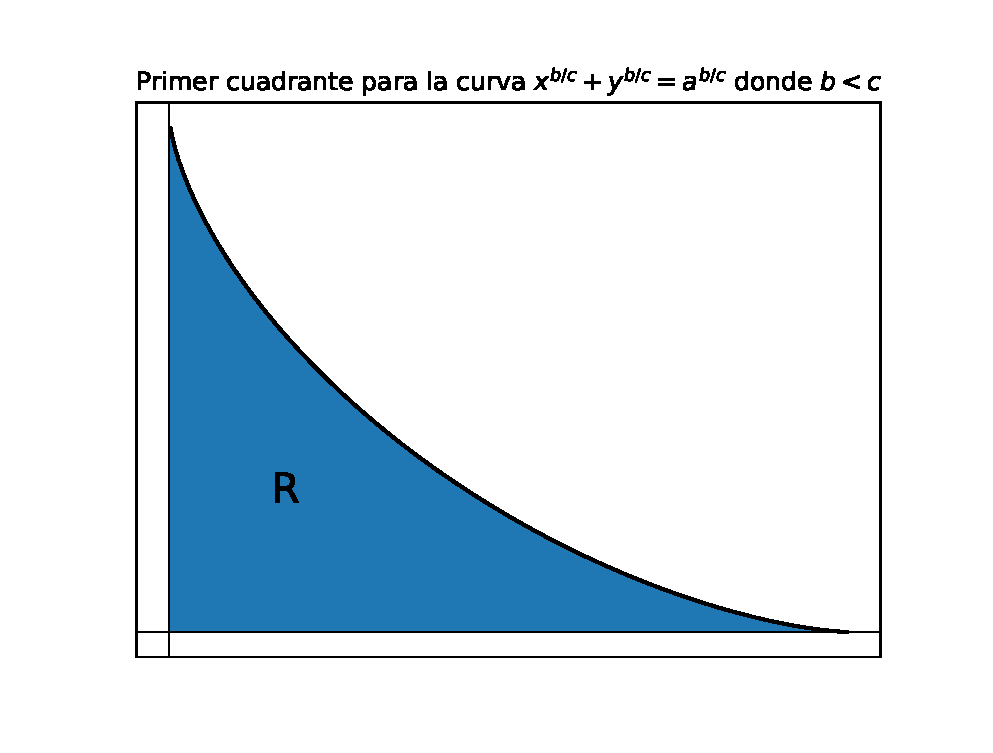
\includegraphics[scale=0.5]{Imagenes/plot_curva_estrella_02.eps}
    \caption{Cuadrante de trabajo para calcular el área.}
    \label{fig:figura_curva_estrella_cuadrante}
\end{figure}
\end{frame}
\begin{frame}
\frametitle{Solución al problema}
\setbeamercolor{item projected}{bg=blue!70!black,fg=yellow}
\setbeamertemplate{enumerate items}[circle]
\begin{enumerate}[<+->]
\item Obtendremos inicialmente una solución general para valores $a$, $b$ y $c$.
\item Posteriomente calcularemos la solución particular con los valores que nos da el enunciado: $b = 2$ y $c = 3$.
\end{enumerate}
\end{frame}
\begin{frame}
\frametitle{Previo a la solución}
Tenemos entonces que:
\begin{align*}
\mbox{Área = } 4 \iint \limits_{R} \dd{A}
\end{align*}
donde $R$ representa la región en el primer cuadrante rodeado por la curva y los ejes, revisa la figura (\ref{fig:figura_curva_estrella_cuadrante}).
\end{frame}
\begin{frame}
\frametitle{Detallando la integral a resolver}
Pasamos de la integral doble a una integral doble equivalente con límites:
\begin{align*}
A = 4 \int_{0}^{a} \dd{x} \, \int_{0}^{\left( a^{\frac{b}{c}} - x^{\frac{b}{c}} \right)^{\frac{c}{b}}} \dd{y}
\end{align*}
\end{frame}
\begin{frame}
\frametitle{Cambio de variable para $y$}
Para evaluar la integral en $y$, hacemos el siguiente cambio de variable:
\begin{align*}
y = a \, v^{\frac{c}{b}} \hspace{1cm} \Longrightarrow \hspace{1cm} \dd{y} = a \, \left( \dfrac{c}{b} \right) \, v^{\frac{c}{b} - 1} \dd{v}
\end{align*}
\end{frame}
\begin{frame}
\frametitle{Cambio de variable para $x$}
Mientras estamos en eso, también podemos hacer el mismo tipo de cambio en la variable para $x$:
\begin{align*}
x = a \, u^{\frac{c}{b}} \hspace{1cm} \Longrightarrow \hspace{1cm} \dd{x} = a \, \left( \dfrac{c}{b} \right) \, u^{\frac{c}{b} - 1} \dd{u}
\end{align*}
\end{frame}
\begin{frame}
\frametitle{Nuevos límites de integración}
Al realizar los cambios de variables, corresponde entonces también realizar el cambio en los límites de integración, por lo tanto:
\begin{align*}
A = \dfrac{4 \, a^{2} \, c^{2}}{b^{2}} \, \int_{0}^{1} u^{\frac{c}{b} - 1} \dd{u} \, \int_{0}^{1-u} v^{\frac{c}{b} - 1} \dd{v}
\end{align*}
\end{frame}
\begin{frame}
\frametitle{Integrando con respecto a $v$}
Al realizar la integración con respecto a $v$, tenemos:
\begin{align*}
A = 4 \, a^{2} \, \left( \dfrac{c}{b} \right) \, \int_{0}^{1} u^{\frac{c}{b} - 1} (1 - u)^{c/b} \dd{u}
\end{align*}
\pause
Recordando que la función Beta se define como:
\begin{align*}
B(x, y) = \int_{0}^{1} t^{x-1} (1 - t)^{y-1} \dd{t} \hspace{1cm} x > 0, y > 0
\end{align*}
\end{frame}
\begin{frame}
\frametitle{Resultado parcial}
Encontramos una buena utilidad para las funciones que involucran integrales, ya que el cálculo de éstas se simplifica mucho.
\\
\bigskip
\pause
Entonces la integral anterior en la expresión para el área $A$, es la integral Beta, por tanto:
\end{frame}
\begin{frame}
\frametitle{Resultado parcial}
Tenemos que:
\begin{align*}
A = 4 \, \left( \dfrac{c}{b} \right) \, a^{2} \, B \left( \dfrac{c}{b}, \dfrac{c}{b} + 1 \right)
\end{align*}
\pause
Para resolver la expresión en términos mucho más sencillos, debemos de ocupar las propiedades e identidades para las funciones Gamma y Beta, como veremos a continuación:
\end{frame}
\begin{frame}
\frametitle{Ocupando propiedades}
Conocemos una expresión que relaciona la función Beta con la Gamma:
\begin{align*}
B (x, y) = \dfrac{\Gamma (x) \, \Gamma (y)}{\Gamma (x + y)}
\end{align*}
Que podemos ocupar en el resultado anterior.
\end{frame}
\begin{frame}
\frametitle{Ocupando propiedades}
Así tenemos que:
\begin{align*}
A &= 4 \, \left( \dfrac{c}{b} \right) \, a^{2} \, B \left( \dfrac{c}{b}, \dfrac{c}{b} + 1 \right) \\[0.5em]
A &= 4 \, \left( \dfrac{c}{b} \right) \, a^{2} \, \left[ \dfrac{\mathlarger{\Gamma} \left( \dfrac{c}{b} \right) \, \mathlarger{\Gamma} \left( \dfrac{c}{b} + 1 \right)}{\mathlarger{\Gamma} \left( \dfrac{2 \, c}{b} + 1 \right)} \right]
\end{align*}
\end{frame}
\begin{frame}
\frametitle{Ocupando propiedades}
Seguimos ocupando las identidades de la función Gamma:
\begin{align*}
\mathlarger{\Gamma} (x + 1) &= x \, \mathlarger{\Gamma} (x) \\[0.5em]
\mathlarger{\Gamma} \left( \dfrac{c}{b} + 1 \right) &= \dfrac{c}{b} \, \mathlarger{\Gamma} \left( \dfrac{c}{b} \right) \\[1em]
\mathlarger{\Gamma} \left( \dfrac{2 \, c}{b} + 1 \right) &= \dfrac{2 \, c}{b} \, \mathlarger{\Gamma} \left( \dfrac{2 \, c}{b} \right)
\end{align*}
\end{frame}
\begin{frame}
\frametitle{Solución general}
La solución general para el área contenida en el astroide es:
\begin{align*}
A &= 4 \, \left( \dfrac{c}{b} \right) \, a^{2} \, \left[ \dfrac{\mathlarger{\Gamma} \left( \dfrac{c}{b} \right) \, \mathlarger{\Gamma} \left( \dfrac{c}{b} + 1 \right)}{\mathlarger{\Gamma} \left( \dfrac{2 \, c}{b} + 1 \right)} \right] \\[1em]
A &= \dfrac{\mathlarger{\Gamma} \left( \dfrac{c}{b} \right) \, \mathlarger{\Gamma} \left( \dfrac{c}{b} \right)}{\mathlarger{\Gamma} \left( \dfrac{2 \, c}{b} \right)} \, \left( \dfrac{2 \, c \, a^{2}}{b} \right)
\end{align*}
\end{frame}
\begin{frame}
\frametitle{Solución general}
Por lo que tenemos una expresión más sencilla que involucra la evaluación de la función Gamma, para cualesquiera valores de $b$ y $c$.
\begin{align*}
A = \dfrac{\mathlarger{\Gamma} \left( \dfrac{c}{b} \right) \, \mathlarger{\Gamma} \left( \dfrac{c}{b} \right)}{\mathlarger{\Gamma} \left( \dfrac{2 \, c}{b} \right)} \, \left( \dfrac{2 \, c \, a^{2}}{b} \right)
\end{align*}
\end{frame}
\begin{frame}
\frametitle{Solución particular}
El área del astroide cuando $b = 2$ y $c = 3$ es:
\begin{eqnarray*}
A &=& \dfrac{\mathlarger{\Gamma} \left( \dfrac{3}{2} \right) \, \mathlarger{\Gamma} \left( \dfrac{3}{2} \right)}{\mathlarger{\Gamma} (3)} \, (2) \left( \dfrac{3}{2} \right) \, a^{2} = \\[1em] \pause
&=& \dfrac{\dfrac{\sqrt{\pi}}{2} \, \dfrac{\sqrt{\pi}}{2}}{2} \, 3 \, a^{2} = \\[1em] \pause
&=& \dfrac{3 \, a^{2} \, \pi}{8} \qed
\end{eqnarray*}
\end{frame}
\end{document}